% Chapter 3

\chapter{DESIGN \& ARCHITECTURE}

% \begin{figure}[hbt] 
% \begin{center}
% \includegraphics[scale=.40]{./figures/bddig1}
% \caption{\label{fig:BDDD}A BDD where some boolean variables occur more than
% once on an evaluation path.}
% \end{center}
% \end{figure}

We propose a design quality assessment system based on Machine learning models that utilizes an abstract syntax tree (AST) to represent programs. The ML models are regression model that are trained on assessed student programs to predict a score between zero and one. Each feature a model uses is designed to be meaningful to human interpretation and is based on statistics collected from the program’s AST. We intentionally do not use deep learning as it would make the representation of the program difficult to understand. Personalized feedback is generated based on each feature of an individual program. By swapping a feature’s value for an individual program with the average feature value of good programs, it is possible to determine which changes need to be made to the program to improve design


\section{TRAINING} 

Dataset contains the code and corresponding scores for each of the student codes. Features from code were extracted by using two ways. Some features were extracted directly from the code. For the other features, the code was first transformed into an Abstract Syntax Tree(AST) then the features were extracted from the AST. The extracted features were used to train the model. Three models were trained separately: Support vector regressor, Random forest and Multi layer perceptron. The models trained were all regression models which were trained to predict the scores that should be given to the evaluated codes. 

\begin{figure}[h]
\centering
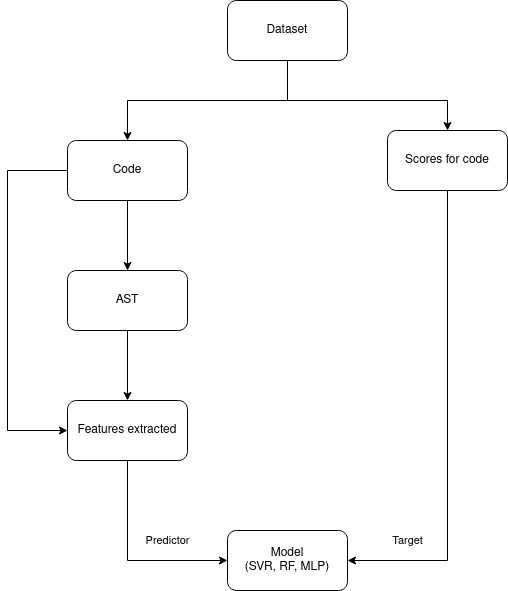
\includegraphics[width=0.9\textwidth]{./training.jpg}
\caption{Training}
\label{fig1}
\end{figure}

\newpage

\section{DEPLOYMENT} 

The student code is input. Features are extracted from the code as explained in the section above. Some features are extracted from the code itself and the rest from an AST representation of the code. This feature set is input into the trained models from the previous section. The model predicts a score for the input code based on the feature set.

In order to avoid the need for a dataset with explicit feedback annotation, we use our model, trained on predicting design score, to evaluate how changes in program features would lead to a higher assessed score. Using the training data, we compute an average feature vector x of all the “good” programs. To generate feedback for a program, its feature vector is compared to the average.

\begin{figure}[h]
\centering
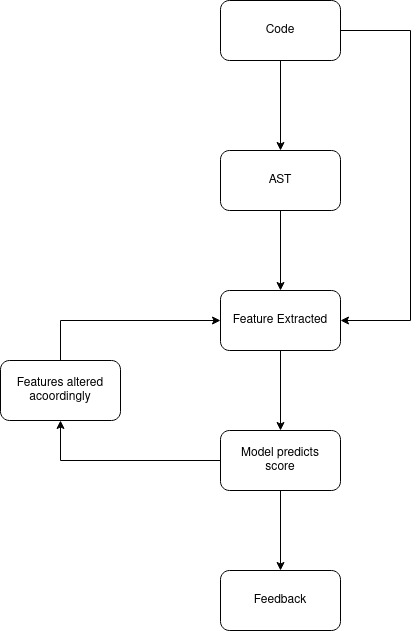
\includegraphics[scale=0.7]{./Deployment.jpg}
\caption{Deployment}
\label{fig1}
\end{figure}